% Chapter Template

\chapter{Sensory Redundancy: Are two heads better than one?} % Main chapter title

\label{Chapter4} % Change X to a consecutive number; for referencing this chapter elsewhere, use \ref{ChapterX}

\lhead{Chapter 4. \emph{Sensory Redundancy: Are two heads better than one?}} % Change X to a consecutive number; this is for the header on each page - perhaps a shortened title

%----------------------------------------------------------------------------------------
%	SECTION 1
%----------------------------------------------------------------------------------------

\section{Why have one sensor when two are better?}
A key part of the human experience is that it is multisensory. In \cite{barsalou2008grounded}, Lawrence Barsalou speaks about how multisensory processing aids human cognition in a number of ways. Firstly, multisensory information aids in the classification of experiences by providing additional and complimentary information that is not accounted for in only a single modality. 

The Mcgurk effect \cite{mcgurk1976hearing} demonstrates how the visual stimuli of lip reading affects the classification of heard sounds. Whilst this effect can lead to incorrect classifications when misaligned data is provided e.g. utterances of the syllable [ba] dubbed on to lip movements for [ga], lead to normal adults hearing [da]; in normal circumstances i.e. when two people are speaking to one and other, lip reading aids in classifying heard sounds \cite{ma2009lip}. This is particularly importnant in noisy environments, which leads to another of Barsalou's ideas about multisensory processing: information redundancy.

The reason that lip reading can aid hearing in noisy evironments is that it provides an additional vector along which the human brain can reconstruct missing information. I.e. when something is mis-heard due to background noise, the visual information gained from looking at the face of the speaker can be used to reconstruct their utterance.

The ability to reconstruct missing data from a secondary modality has not only been seen in humans \cite{ma2009lip, samuel1997lexical} but has been demonstrated in computational modals for example, Ngiam et al.\cite{ngiam2011multimodal}.

In order to be able to reconstruct missing data from a secondary modality, symbol grounding needs to have occured, i.e. the meaning of a percept in modality A must be known in modality B.
If both the forward and inverse relationship between modalities is known, then bidirectional symbol grounding has occured and we are able to reconstruct modality A from modality B and modality B from modality A.

In this chapter I will explore these two ideas, improved classification and reconstruction of missing information through  bidirectional symbol grounding using multimodal autoencoders (MAE).



\section{Generating images from natural language}
\subsection{Aims}
The experiment in this section looks at whether having access to a second modality improves classification accuracy over the baseline accuracy of classification of either of the two individual modalities as well as how well missing data can be reconstructed from a secondary modality.

\subsection{UCU Arabic Spoken Digits and MNIST} 
\label{sec:UCU}
This experiment utilises two datasets, UCU Arabic Spoken Digits and MNIST Handwritten Digits.

\subsubsection{UCU Arabic Spoken Digits}
UCU Arabic Spoken Digits (UCU) is a dataset containing the 13 Mel Frequency Cepstrum Coefficients representing the audio of the digits 0 to 9 being said by 88 different speakers \cite{hammami2009tree,hammami2010improved}. It contains 8800 utterances (10 digits x 10 repetitions x 88 speakers). Audio was sampled at 11025Hz.

As utterances are not of a fixed length, it is necessary to pad the utterances to be equal length. The longest utterance in the dataset contains 93 samples. For ease of downsampling within the neural network, we pad all uttereances to be 100 samples long by appending zeros. We also pad each sample to contain 16 features, the 13 MFCCs and 3 zeros to further facilitate down sampling\footnote{Downsampling is easier with even numbers of features and samples as we can half the size of the data using strided convolutions, s=(2,2), without worrying about integer division errors e.g. $5/2=2$ but $2\times2 \neq5$}.

As we will be classifying the digits, it is necessary to check that padding the digits does not provide a cheat for this. As such, we analise the mean number of samples for each digit and their standard deviations as depicted in \ref{fig:ucu_dig_length}. We then perform a linear regression on the number of samples to demonstrate that it is not possible to accurately predict a digits class given only the length of the utterance.

\begin{figure}
	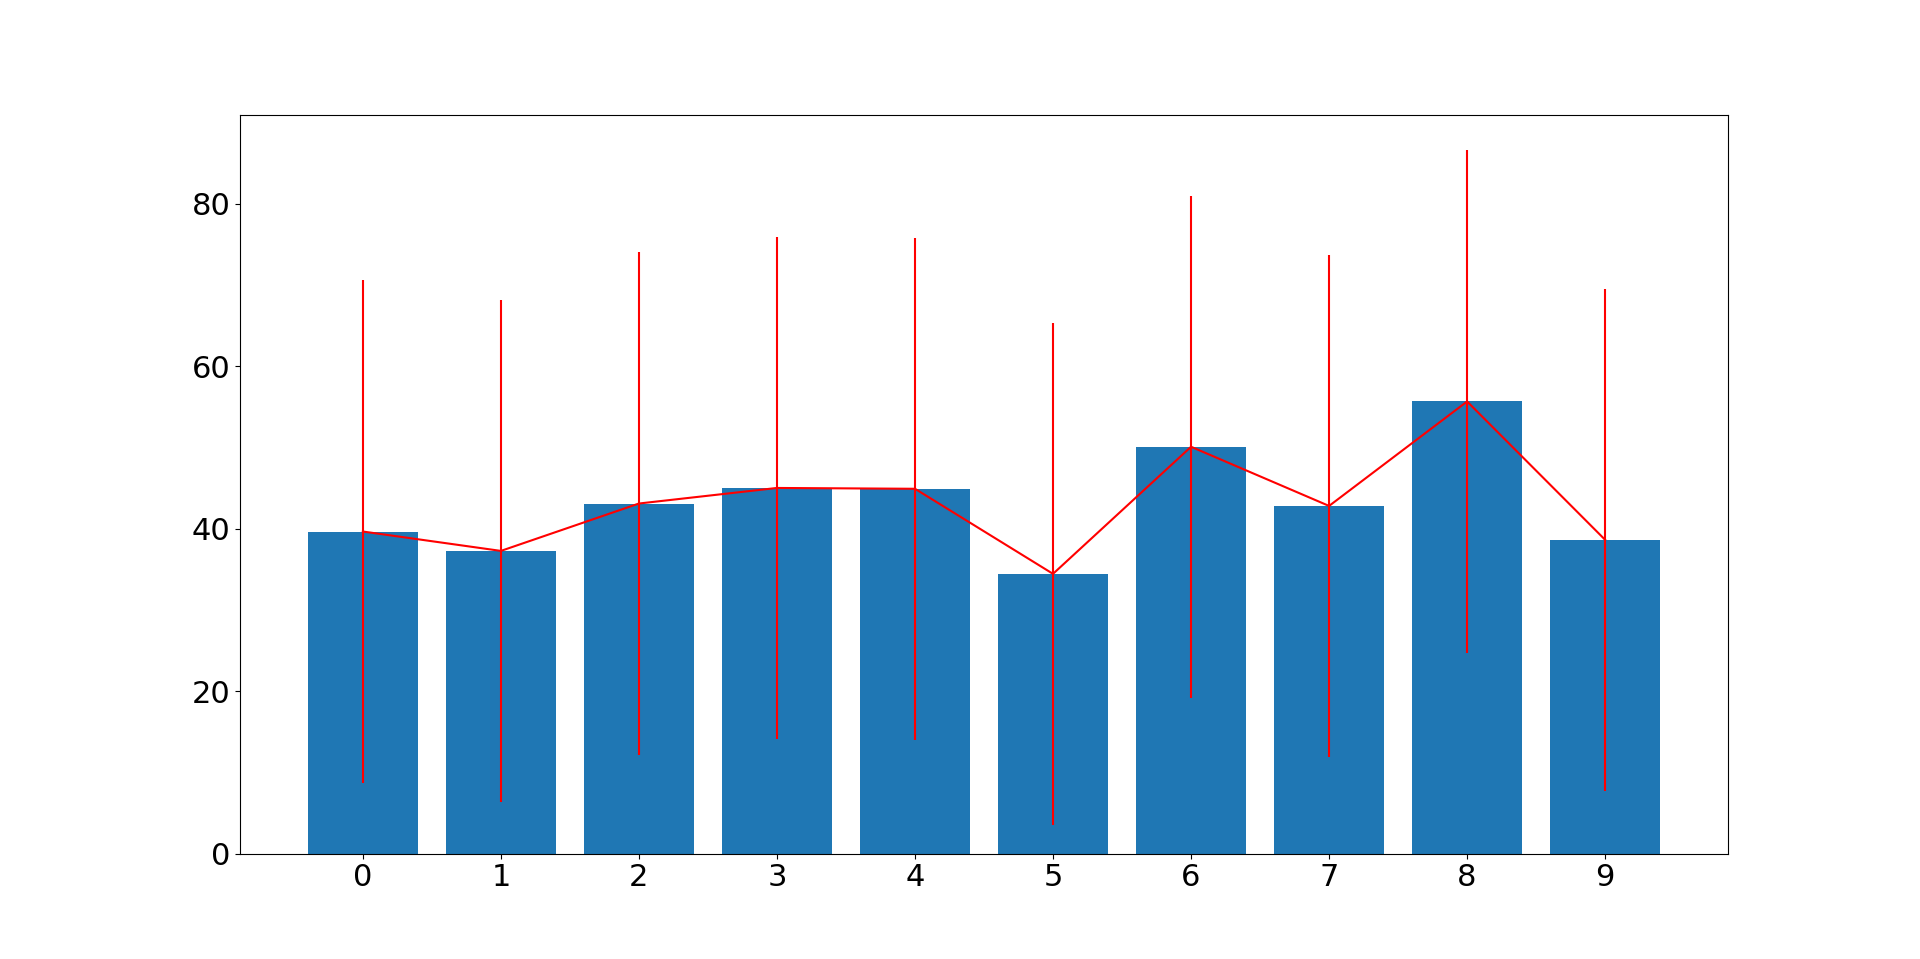
\includegraphics[width=\textwidth]{./Figs/mnistSpoken/UCU_digit_length.png}
	\caption{Mean number of samples for each digit in the UCU Arabic Spoken Digits Dataset. Red bars show the standard devaition in length for each each digit.}
	\label{fig:ucu_dig_length}

\end{figure}

Figure \ref{fig:ucu_dig_length} shows the mean number of samples for each digit in the UCU dataset. Whilst there is a difference in the mean length of each digit, the standard deviation for each digit is relatively large as can be seen in table \ref{tab:UCU_sampLen}. Therefore, trying to classifiy the digits just by the number of samples in an example, would be ineffective.

	\begin{table}
		\centering
		\begin{tabular}{|c|c|c|}
			\hline
			Digit & Mean Length (samples) & Standard Deviation \\ \hline
			0 & 39.66 & $\mypm 29.25$ \\ \hline
			1 & 37.27 & $\mypm 25.58$ \\ \hline
			2 & 43.11 & $\mypm 31.43$ \\ \hline
			3 & 45.02 & $\mypm 34.05$ \\ \hline
			4 & 44.92 & $\mypm 31.63$ \\ \hline
			5 & 34.44 & $\mypm 23.63$ \\ \hline
			6 & 50.10 & $\mypm 35.90$ \\ \hline
			7 & 42.81 & $\mypm 30.41$ \\ \hline
			8 & 55.67 & $\mypm 41.01$ \\ \hline
			9 & 38.63 & $\mypm 30.94$ \\ \hline

		\end{tabular}
		\caption{Mean length and standard deviation of digits in the UCU dataset.}
		\label{tab:UCU_sampLen}
	\end{table}


Performing a linear regression on the number of samples for each digit versus its class, we get an accuracy of 6.18\% when classifying the test set.

\subsubsection{MNIST Handwritten Digits}
MNIST Handwritten Digits (MNIST) is a well known and ofte used dataset in the machine learning community. It contains 60000 training samples and 10000 test samples, evenly split between the digits 0 to 9. 
Each digit is presented as a grey-scale, 28x28 pixel image \cite{lecun1998mnist}. 

\subsection{Problem Description}
The experiments with these datasets will explore two problems, classification and bidirectional symbol grounding. 

\subsubsection{Classification}
Each of the utterances or images from the UCU or MNIST datasets are classified as being a numeric digit, 0 to 9. By combining both datasets, we can explore whether the addition of a second modality enhances overall classification accuracy.

I start off exploring the classification abilities of neural networks by performing a linear regression with a single, dense neural network layer with a softmax activation on the embedding of an autoencoder. To generate baseline classifications accuracies for each dataset, I use autoencoders for each dataset separately.

Once a classification baseline has been established for each dataset, I make use of a multimodal autoencoder, using paired examples from each dataset to train it.

\subsubsection{Bidirectional Symbol Grounding}

I demonstrate that a neural network can perform bidirectional symbol grounding \cite{barsalou2008grounded} when presented with aligned images and utterances. To explore this, I show how a MAE can learn to reconstruct the correct image of a digit given an utterance as well as MFCCs which have a small mean squared error from the correct utterance given an image of a digit. This shows that an internal symbolic language has been learnt in the form of the latent embedding created by the encoders of the MAE.


\subsection{Experiment Details}
\subsubsection{Dataplumbing}
Images from the MNIST dataset are kept at their original scale of 28x28 pixels and are normalised such that each pixel has a value from 0 to 1 based on it's intensity, with zero equating to black and 1 being white.

The UCU dataset is normalised so that all MFCCs take a value from 0 to 1 based on the value of the MFCC such that the highest value is 1 and the lowest 0. Utterances are padded to be 100x16 as previously described.

\paragraph{Combining Datasets}
\label{sec:UCU_mnist_comb}
Due to the difference in size between the datasets, 8,800 samples for UCU and 80,000 samples for MNIST, I randomly sample from the UCU dataset and pair this with a sample from MNIST. This means that each sample from UCU is repeated approxiamtely 9.1 times ($80000/8800=9.0909$).

\paragraph{Merging Modalities}
In order to combine the two different modalities, I explore different merging techniques: Concatenation (\textit{Concat}) and Addition (\textit{Add}). To do this, the embeddings of both modalities are ensured to have the same shape and then are merged using the methods described in Equations \ref{eqn:concat} and \ref{eqn:add}, concatenation and addition, respectively. %and \ref{eqn:xply}.

 \begin{equation}
 	merged = im_i^{emb} || mfcc_i^{emb}
 	\label{eqn:concat}
 \end{equation}

 \begin{equation}
 	merged = im_i^{emb} + mfcc_i^{emb}
 	\label{eqn:add}  
 \end{equation}
 
  %\begin{equation}
 	%merged = x1^*_i * x2^*_i
 	%\label{eqn:xply}  
 %\end{equation}

Where $im_i^{emb}$ and $mfcc_i^{emb}$ represent the embeddings, output by the image and MFCC encoders respectively for image and MFCC inputs $im_i$ and $mfcc_i$.

\subsubsection{Training Procedures}

The MAEs are trained in two different ways for both types of merging, these are referred to as bimodal (Bi) and randomly degraded (RD).

\paragraph{Bimodal}
Under the bimodal (Bi) training procedure, the MAE is presented with bimodal input for all training instances. That is, both image and MFCC inputs are present for all inputs and the MAE is trained to reproduce this input as its output.

\paragraph{Randomly Degraded}
Under the randomly degraded (RD) training procedure, one third of image inputs are removed at random and a third of MFCC inputs are removed at random. It is ensured that each training instance always has at least one input modality present. That is, a training instance never has both its image and MFCC input removed. 

The removed modality is replaced with an array of zeros of the same shape as the original input (28x28 for the image and 100x16 for MFCCs).

The MAE is then trained to reproduce both the image and MFCCs regardless of whether one of these has been ommited from the input.

\subsubsection{Testing Conditions}
Each MAE (Concatenate and Addition) was tested in three different ways, bimodal, image only and MFCC only.

\paragraph{Bimodal}
In the bimodal (bi) testing condition both image and MFCC data are used as input for each testing instance and we are interested in observing the classification accuracy as well as the total regeneration loss.

\paragraph{Image Only}
In the image only (Im) testing condition, only images are provided as input data. We are interested in the classification accuracy as well as the MFCC reconstruction loss. We are not interested in the image reconstruction loss, as it is expected that, as the image is provided as input this will be low (which it is for all models and training procedures as seen in table \ref{tab:mnist_ucu_master_res}).  

\paragraph{MFCC Only}
Similarly to the image only condition, the MFCC only (MFCC) condition provides only MFCCs as input and we are interested in the classification accuracy as well as the image reconstruction loss. We are not interested in the MFCC regeneration loss as MFCCs are given as input it will be low (which it is for all models and training procedures as seen in table \ref{tab:mnist_ucu_master_res}).  

\subsubsection{Network Description}
\paragraph{Baseline Models}
To generate the baseline classification accuracies for both the UCU and MNIST data, I make use of unimodal autoencoders. The descrition of the autoencoder for the MNIST dataset can be found in table \ref{tab:MNIST_AE_description} and the autoencoder for the UCU dataset in table \ref{tab:UCU_AE_description}.

	\begin{table}[t]
		\centering
		\begin{tabular}{|c|c|c|c|c|c|c|}
			\hline
			Block & Layer & Type & Neurons & Kernel & Strides & Activation  \\ \hline
			\multirow{4}{*}{Encoder} & 1	&	2D Conv & 32 & (3,3) & (1,1)  & Relu\\ \cline{2-7}
			& 2	&	2D Conv & 64 & (3,3) & (2,2) & Relu \\ \cline{2-7}
			& 3	&	2D Conv & 64 & (3,3) & (2,2) & Relu \\ \cline{2-7}
			& 4 	&	Dropout p=0.25 &	 & 	     &       & \\ \hline
			Embedding & 5	&	2D Conv & 32 & (3,3) & (1,1) & Relu \\ \hline
			Classifier & 6c	&	Dense          & 10 &       &       & Softmax      \\ \hline
			\multirow{5}{*}{Decoder}& 6 	&	Dropout p=0.25 &	 & 	     &       & \\ \cline{2-7}
			& 7	&	2D Trans Convn & 64 & (3,3) & (2,2) & TanH \\ \cline{2-7}
			& 8	&	2D Transp Conv & 64 & (3,3) & (2,2) & TanH \\ \cline{2-7}
			& 9	&	2D Trans Conv & 32 & (3,3) & (1,1) & TanH \\ \cline{2-7}
			& 10	&	2D Trans Conv & 1 & (3,3) & (1,1) & Sigmoid \\ \hline
		\end{tabular}
		\caption{Image autoencoder and classifier. Layer 6c performs classification, whilst the branch starting at layer 6 regenerates the image.}
		\label{tab:MNIST_AE_description}
	\end{table}

	\begin{table}[t]
		\centering
		\begin{tabular}{|c|c|c|c|c|c|c|}
			\hline
			Block & Layer & Type & Neurons & Kernel & Strides & Activation  \\ \hline
			\multirow{5}{*}{Encoder} & 1	&	2D Conv & 32 & (3,3) & (1,1)  & Relu\\ \cline{2-7}
			& 2	&	2D Conv & 64 & (3,3) & (2,2)  & Relu\\ \cline{2-7}
			& 3 	&	Dropout p=0.25 &	 & 	     &        & \\ \cline{2-7}
			& 4	&	Dense          & 3136 & 	 &        & \\ \cline{2-7}
			& 5   &	Reshape (7,7,64) &    &     &        & \\ \hline
			Embedding & 6	&	2D Conv & 32 & (3,3) & (1,1)  & Relu  \\ \hline
			Classifier & 7c	&	Dense          & 10 &       &        & Softmax \\ \hline
			\multirow{7}{*}{Decoder} & 7 	&	Dropout p=0.25 &	 & 	     &        & \\ \cline{2-7}
			& 9	&	Dense			& 3200 &     &        & \\ \cline{2-7}
			& 10	&	Reshape (25,4,32) &    &    &        & \\ \cline{2-7}
			& 11	&	2D Trans Conv & 64 & (3,3) & (2,2)  & TanH \\ \cline{2-7}
			& 12	&	2D Trans Conv & 64 & (3,3) & (2,2)  & TanH \\ \cline{2-7}
			& 13	&	2D Trans Conv & 32 & (3,3) & (1,1)  & TanH \\ \cline{2-7}
			& 14	&	2D Trans Conv & 1 & (3,3) & (1,1) & Sigmoid \\ \hline
		\end{tabular}
		\caption{MFCC autoencoder and classifier. Layer 7c performs classification, whilst the branch starting at layer 7 regenerates the MFCCs. The addition of reshape layers is to ensure the final shape of the regenerated MFCCs matches the target shape whilst the embedding shape matches that of the embedding of the image autoencoder.}
		\label{tab:UCU_AE_description}
	\end{table}

\paragraph{Multimodal Autoencoder}
By combining the two autoencoders described in tables \ref{tab:MNIST_AE_description}, \ref{tab:UCU_AE_description}, a multimodal autoencoder is created. The embeddings from each of the unimodal autoencoders are merged by either, concatenation or addition.
 
	\begin{table}
		\centering
		\begin{tabular}{|c|c|c|c|c|c|c|}
			\hline
			Block & Layer & Type & Neurons & Kernel & Strides & Activation \\ \hline
			\multirow{2}{*}{Image} & 1i	&	2D Conv & 32 & (3,3) & (1,1) & Relu \\ \cline{2-7}
			& 2i	&	2D Conv & 64 & (3,3) & (2,2) & Relu \\ \cline{2-7}
			\multirow{2}{*}{Encoder}& 3i	&	2D Conv & 64 & (3,3) & (2,2) & Relu \\ \cline{2-7}
			& 4i	&	Dropout p=0.25 &	 & 	     &       &  \\ \hline

			\multirow{3}{*}{MFCC} & 1m	&	2D Conv & 32 & (3,3) & (1,1) & Relu \\ \cline{2-7}
			& 2m	&	2D Conv & 64 & (3,3) & (2,2) & Relu \\ \cline{2-7}
			& 3m 	&	Dropout p=0.25 &	 & 	     &       & \\ \cline{2-7}
			\multirow{2}{*}{Encoder} & 4m	&	Dense          & 3136 & 	 &       & \\ \cline{2-7}
			& 5m  &	Reshape (7,7,64) & & & & \\ \hline

			Merge & 6im	& Merge & & & & \\ \hline
			Embedding& 7im	&	2D Conv & 32 & (3,3) & (1,1) & Relu \\ \hline
			Classifier & 8c	&	Dense          & 10 &       &       & Softmax \\ \hline

			\multirow{3}{*}{Image} & 8i 	&	Dropout p=0.25 &	 & 	     &       & \\ \cline{2-7}
			& 9i	&	2D Trans Conv & 64 & (3,3) & (2,2)  & TanH \\ \cline{2-7}
			& 10i	&	2D Trans Conv & 64 & (3,3) & (2,2)  & TanH \\ \cline{2-7}
			\multirow{2}{*}{Decoder}& 11i	&	2D Trans Conv & 32 & (3,3) & (1,1)  & TanH \\ \cline{2-7}
			& 12i	&	2D Trans Conv & 3 & (3,3) & (1,1) & Sigmoid\\ \hline 

			\multirow{4}{*}{MFCC} & 8m 	&	Dropout p=0.25 &	 & 	     &        & \\ \cline{2-7}
			& 9m	&	Dense			& 3200 & &           & \\ \cline{2-7}
			& 10m	&	Reshape (25,4,32) & & & &\\ \cline{2-7}
			& 11m	&	2D Trans Conv & 64 & (3,3) & (2,2)  & TanH \\ \cline{2-7}
			\multirow{3}{*}{Decoder}& 12m	&	2D Trans Conv & 64 & (3,3) & (2,2)  & TanH \\ \cline{2-7}
			& 13m	&	2D Trans Conv & 32 & (3,3) & (1,1)  & TanH \\ \cline{2-7}
			& 14m	&	2D Trans Conv & 1 & (3,3) & (1,1)  & Sigmoid\\ \hline
		\end{tabular}
		\caption{Image and MFCC multimodal autoencoder. Layers marked i, m, im and c are image, MFCC, image and MFCC and classification respectively.}
		\label{tab:UCU_MNIST_MAE_description}

	\end{table}




\subsection{Results}

\subsubsection{Classification Results}
Table \ref{tab:mnist_ucu_master_res} shows the complete results for all of the experiments run on the combined UCU and MNIST dataset. For convenience, this table is broken down into three other tables, \ref{tab:mnist_ucu_bi_res} for the bimodal testing condition, \ref{tab:mnist_ucu_im_res} for the image only condition and \ref{tab:mnist_ucu_mfcc_res} for the MFCC only testing condition. 

All results reported here are the mean of a four-fold cross validation. That is, each training and testing condition was run four times and the average results are shown.

\begin{table}
	\centering
		\begin{tabular}{|c|c|c|c|c|c|c|c|}
		\hline
		Model & Training & Testing & Im MSE & MFCC MSE & Lb MSE & Total MSE & Acc \\
		\hline
		Image AE & Im & Im & 0.0027	&	&0.0019	& 0.0046	&	0.9883\\ \hline
		MFCC AE & MFCC & MFCC & 	&0.0113	&	0.0026	&	0.0139	& 0.9832\\ \hline
		\multirow{6}{*}{Add MAE} & \multirow{3}{*}{Bi} & Bi &	0.0030	&	0.0401	&	0.0006	&	0.0437	&0.9967\\ \cline{3-8}
		&& Im &	0.0076	&	0.1641	&	0.0763	&	0.2479	&0.4501 \\ \cline{3-8}
		&& MFCC &	0.1138	&	0.0399	&	0.0057	&	0.1594	&0.9624 \\ \cline{2-8}
		& \multirow{3}{*}{RD} & Bi&	0.0033	&	0.0176	&	0.0001	&	0.0210	& 0.9993 \\ \cline{3-8}
		&& Im &	0.0027	&	0.0455	&	0.0025	&	0.0508	& 0.9834\\ \cline{3-8}
		&& MFCC & 0.0556	&	0.0166	&	0.0031	&	0.0752	&	0.9789 \\ \hline
		
		\multirow{6}{*}{Concat MAE} & \multirow{3}{*}{Bi} & Bi &	0.0031	&	0.0423	&	0.0009	& 0.0462	&	0.9945 \\ \cline{3-8}
		&& Im &	0.0055	&	0.2029	&	0.0843	&	0.2927	&	0.3496 \\ \cline{3-8}
		&& MFCC &0.1138	&	0.0420	&	0.0079	&0.1637	&	0.9455 \\ \cline{2-8}
		& \multirow{3}{*}{RD} & Bi &	0.0030	&	0.0426	&	0.0002	&	0.0458	&0.9986 \\ \cline{3-8}
		&& Im &	0.0026	&	0.0737	&	0.0026	& 0.0788	&	0.9834
\\ \cline{3-8}
		&& MFCC &	0.0554	&	0.0416	&	0.0026	&	0.0996	&0.9827
 \\ \hline
		\end{tabular}
		\caption{Results from the combined MNIST Handwritten Digits and UCU Arabic Spoken Digits}
		\label{tab:mnist_ucu_master_res}

\end{table}


\begin{table}
	\centering
		\begin{tabular}{|c|c|c|c|c|}
		\hline
		Model & Training & Im MSE & MFCC MSE &  Acc \\ \hline
				Image AE & Im & 	\textbf{0.0027}	&	       			& 	0.9883			\\ \hline		
				MFCC AE & MFCC & 		    		& 	\textbf{0.0113} &	0.9832			\\ \hline		
\multirow{2}{*}{Add MAE} & Bi & 	0.0030			&	0.0401			&	0.9967			\\ \cline{2-5}
						  & RD &	0.0033			&	0.0176			&	\textbf{0.9993}	\\ \hline	
		
\multirow{2}{*}{Concat MAE} & Bi & 0.0031			&	0.0423			&	0.9945			\\ \cline{2-5}		
							 & RD & 0.0030			&	0.0426			&	0.9986			\\ \hline
		\end{tabular}
		\caption{Results from the combined MNIST Handwritten Digits and UCU Arabic Spoken Digits for the bimodal only testing condition.}
		\label{tab:mnist_ucu_bi_res}

\end{table}

In table \ref{tab:mnist_ucu_bi_res} it can be seen that both Concatenate and Addition merging produce models with better prediction accuracy than the baseline models, regardless of training procedure.

\begin{table}
	\centering
		\begin{tabular}{|c|c|c|c|}
		\hline
		Model & Training &  MFCC MSE &  Acc \\ \hline
		Image AE & Im 		&  		    			& \textbf{0.9883}	\\ \hline		
\multirow{2}{*}{Add MAE} & Bi & 	0.1641			& 0.4501 			\\ \cline{2-4}
						  & RD & \textbf{0.0455}	& 0.9834 			\\ \hline	
		
\multirow{2}{*}{Concat MAE} & Bi & 	0.2029		&	0.3496 			\\ \cline{2-4}		
							 & RD & 	0.0737		&	0.9834 			\\ \hline
		\end{tabular}
		\caption{Results from the combined MNIST Handwritten Digits and UCU Arabic Spoken Digits for the image only testing condition.}
		\label{tab:mnist_ucu_im_res}

\end{table}

In comparison to the results shown in table \ref{tab:mnist_ucu_bi_res}, the results in table \ref{tab:mnist_ucu_im_res} show that the MAEs trained using the bimodal training procedure do not generalise well when only a single input modality is available. Where as the MAEs trained using the randomly degraded training procedure perform almost as well as the baseline model. 
\begin{table}
	\centering
		\begin{tabular}{|c|c|c|c|}
		\hline
		Model & Training & Im MSE &  Acc \\ \hline
				
				MFCC AE & MFCC & 					& 	\textbf{0.9832}	\\ \hline		
\multirow{2}{*}{Add MAE} & Bi & 	0.1138			& 	0.9624 			\\ \cline{2-4}
						  & RD &	0.0556			&	0.9789			\\ \hline	
		
\multirow{2}{*}{Concat MAE} & Bi &	0.1138			&	0.9455			\\ \cline{2-4}		
							 & RD & \textbf{0.0554}	& 	0.9827 			\\ \hline
		\end{tabular}
		\caption{Results from the combined MNIST Handwritten Digits and UCU Arabic Spoken Digits for the MFCC only testing condition.}
		\label{tab:mnist_ucu_mfcc_res}

\end{table}

Similarly, the reuslts in \ref{tab:mnist_ucu_mfcc_res} show that the behaviour of the MAEs is very similar under the randomly degraded training procedure regardless of whether it is MFCCs or Images being used as input. However, we see that classification accuracy remains reasonably good under the bimodal training procedure when only MFCCs are present. 

\subsubsection{Reconstruction Results}

In figures \ref{fig:mnistDigits} and \ref{fig:5s} we see examples of reconstructed digits generated by both the Addition and Concatenation MAEs.
\begin{figure}[h]
\begin{center}
	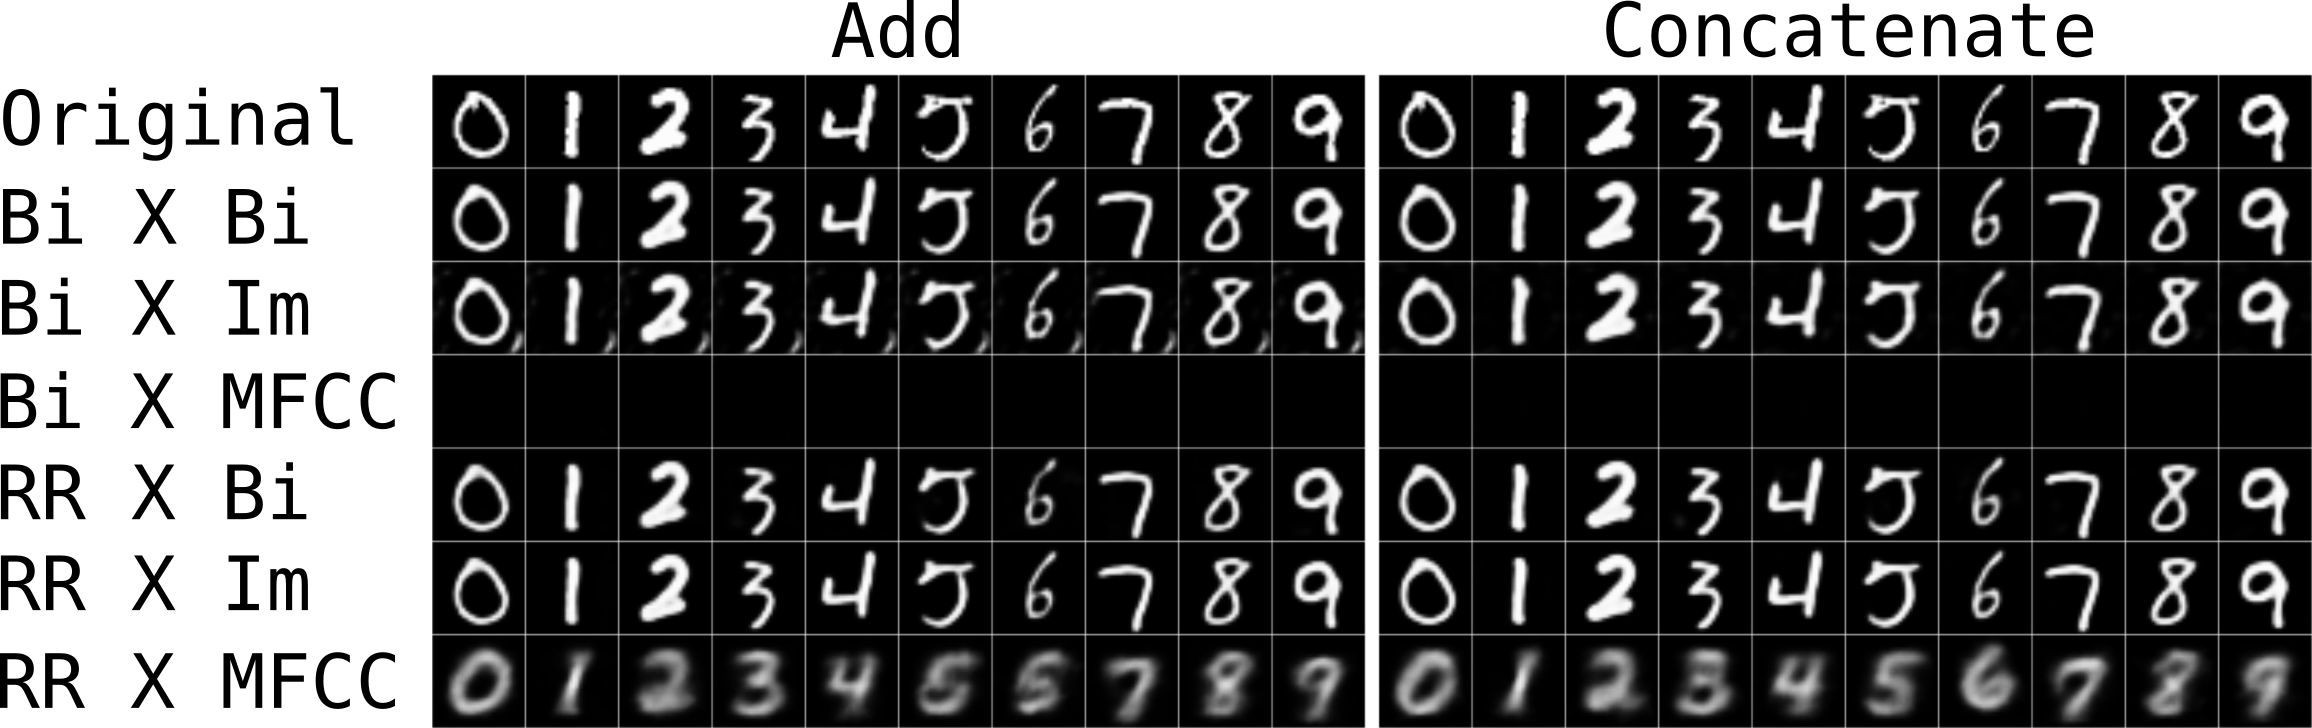
\includegraphics[width=\textwidth]{Figs/mnistSpoken/lbAll.png}
	\caption{A selection of randomly sampled digits generated in different training and testing conditions for both \textit{Add} and \textit{Concat} merging methods.}
	\label{fig:mnistDigits}
\end{center}
\end{figure}

Figure \ref{fig:5s} shows a comparison of two different examples of the digit ``5''. One is (subjectively) poorly written and the other is more prototypical and well formed. We see that under different testing conditions, the MAEs regenerate different ``fives''.
\begin{figure}[h]
\begin{center}
	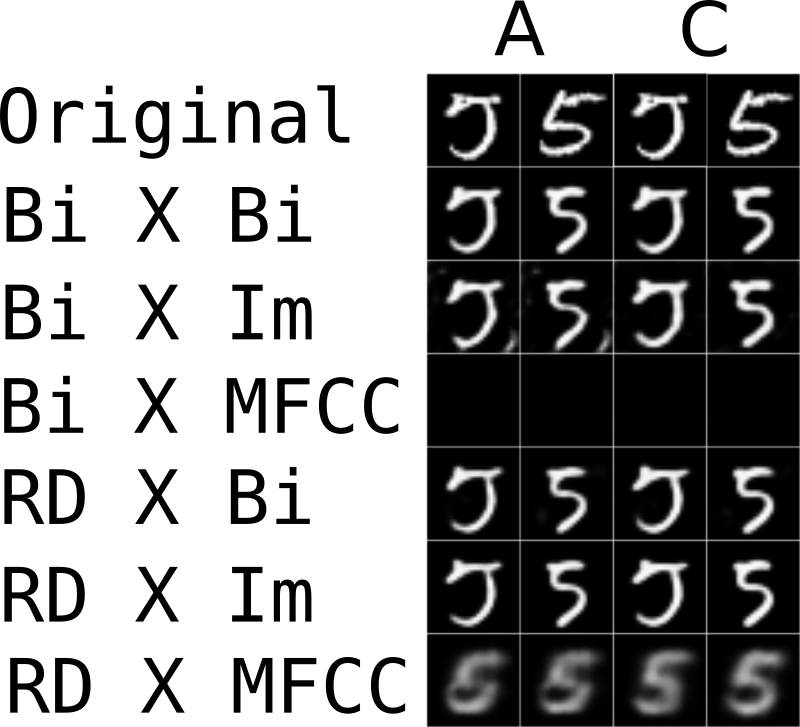
\includegraphics{Figs/mnistSpoken/5s.png}
	\caption{Two examples of the digit 5 being generated in different training and testing conditions for both \textit{Add} and \textit{Concat} merging methoids.}
	\label{fig:5s}
\end{center}
\end{figure}



\subsection{Discussion}

\subsubsection{Discussion of Classification Results}
Looking at table \ref{tab:mnist_ucu_bi_res} we see that both the Add and Concatenate MAEs have better classification accuracy than the baseline, unimodal autoencoder models. However, it is not clear that there is a difference in between the two training procedures, Bimodal and Randomly Degraded.

The difference between the two training procedures becomes clear when we look at table \ref{tab:mnist_ucu_im_res} where we see that the MAEs trained using the Bimodal training procedure have much worse classification rates when presented with only images as input, performing less than half as well as the baseline model, 0.4501 and 0.3496 for the Addition and Concatenation MAEs respectively versus 0.9832 for the baseline image autoencoder.

We also start to see a trade off between unimodal accuracy and mulitmodal accuracy when we look at the Randomly Degraded training procedure MAEs. Whilst both the Addition and Concatenation MAEs outperform the baseline models in the bimodal test condition, they have slightly worse performance when tested in either a unimodal image or MFCC manner. For example, the best performance is given by the Addition MAE under the Randomly Degraded training procedure when both images and MFCCs are present as inputs, with an accuracy of 0.9993. However, if one of the modalities is removed, the accuracy drops to 0.9834 and 0.9789 for image only and MFCC only testing respectively. Comparing this to the baseline unimodal autoencoders, we see classification accuracies of 0.9883 and 0.9832 for image and MFCC autoencoders respectively. 

This means there is a drop of 0.0049 and 0.0043 for image only and MFCC only testing using the Addition MAE. However, this reduction in performance is conterbalanced by the improvement in performnace when both modalities are present, 0.9993 versus the 0.9883 and 0.9832 of the baseline models. This improvement of 0.0110 to 0.0161 over the baseline image and MFCC autoencoders is more than twice the decrease in performance seen when only one modality is available. 

Specifically, the improvement of bimodal classification is 2.2449 times larger than the decrease in performance when only images are available ($0.011 / 0.0049 = 2.2449$). Comparing to the MFCC baseline, the bimodal performance improvement is 3.7442 times larger than the decrease in performance when only MFCCs are available.

\subsubsection{Discussion of Reconstruction Results}
Observing tables \ref{tab:mnist_ucu_bi_res}, \ref{tab:mnist_ucu_im_res} and \ref{tab:mnist_ucu_mfcc_res} we can see that different models had different reconstruction losses (Mean Squared Error). Whilst all MAE models had higher reconstruction losses than the baseline models, this is to be expected. The MAE models are trading off between representing each modality well, whilst the unimodal autoencoders that give the baseline numbers can use their full capacity to minimise the reconstruction loss of their modaility as they do not have to reconstruct the second modality. 

That being said, the image reconstruction loss, is comparable across all MAE models, approximately 0.0031, (see table \ref{tab:mnist_ucu_bi_res} and is very close to the baseline of 0.0027 under the bimodal testing condition (i.e. when the images to be reconstructed are available as input). Further to this, the image reconstruction loss for the MFCC only testing condition is still quite low, though an order of magnitude worse, for the MAEs trained using the Randomly Degraded procedure.

\paragraph{Image reconstruction from MFCCs}
The increase in image reconstruction loss when only MFCCs are provided is due to the construction of an internal symbolic language which represents the meaning of both the utterances but not necessarily their fine details. For example, looking at figure \ref{fig:5s} we see that there are different ways to write the number 5, however both of these images have the same meaning i.e. the symbol ``five''. We should be more interested in preserving this meaning than the minutia of the original images. The same can be said for reconstructing MFCCs, we are more interested in their meaning than their exact enunciation.  

The reconstruction of MFCCs, the reconstruction loss is best for the baseline model but is only 4.0265 times worse for the best performing model on this task. Considering how small the baseline construction error is, being four times worse, is still good performance, especially considering the difficulty of the task.

\paragraph{MFCC reconstruction from Images}
The MFCC reconstruction error is an order of magnitude worse than the image reconstruction error. In part this is due to the nature of the data, as seen by the difference in baseline reconstruction errors. I.e. it appears to be more difficult to reconstruct MFCCs than images, even when MFCCs are given as input.
Another contributing factor to the worse MFCC reconstruction error for the MAEs, is the inbalance between sample numbers for MNIST and UCU. Whilst both datasets are balanced within themselves (there are an equal number fo training samples for each class) there is a big difference between the sizes of MNIST and UCU as discussed previously in section \ref{sec:UCU_mnist_comb}. 

The difference in sizes between the datasets means that reconstructing MFCCs from image inputs will map a large number of inputs to a smaller number of outputs and vice-versa for generating images from MFCC inputs. Therefore images in the test set which look similar to images in the training set, will be mapped to MFCCs similar to those which the training images map too. As there are a smaller number of MFCC examples to map to, our output is less Gaussian. Whilst idealy we would like to map similar looking digits to similar sounding utterances, there is no gaurantee that this is true, either in our dataset or in general. I.e. People with similar handwritting don't necessarily have similar voices. This is simulated by the random assignment of images to MFCCs but this results in discontinuities in the latent space of the network, particularly with respect to generating MFCCs, of which we have fewer examples to capture the true distribution of the data.

Conversely, as there are more examples of images of digits, the distribution of the latent space with respect to the images can get closer to modelling the real distribution of the images. Therefore, given a test MFCC, regardless of whether it is similar to a training MFCC example, its target image, is more likely to be similar to images in the training data.

\paragraph{Effects of randomly degrading inputs}
Figure \ref{fig:mnistDigits} we can clearly see that randomly degrading the training data has a significant effect, beyond just the improvements to classification accuracy seen in tables \ref{tab:mnist_ucu_bi_res}, \ref{tab:mnist_ucu_im_res} and \ref{tab:mnist_ucu_mfcc_res}. Both the Addition and Concatenation MAEs fail to learn to generate images from MFCC data when only bimodal data is presented as training data.

Comparing the images generated by the Add and Concatenate MAEs for the MFCC test condition when the training data has been randomly degraded, we see that the concatenate MAE outperforms the Addition MAE. This is particularly clear when you look at the 5 and 6 generated by the Addition MAE for RD X MFCC, where the MAE has failed to correctly generate a six and has instead generated a five, which is similar to the prototypical five generated when MFCCs for a five are presented.
Unlike the Addition MAE, the Concatenation MAE, correctly generates all digits, including six.

\paragraph{Multiple generations of the same digit}
In figure \ref{fig:5s} we see that different examples of the same digit produce different generation results. Most interestingly however, is that the generated fives shown in the RD X MFCC row, you can see that a more prototypical five is generated from MFCCs than if an image of a non-prototypical five is given. This shows that the meaning of the MFCCs have been grounded in the image modality and that an internal symbolic language has been learnt, i.e. the latent embedding of MFCCs are a symbolic representation which has meaning in both MFCC and image space, hence the ability to generate meaningful images and MFCCs from these embeddings.

\section{Conclusion}
Whilst multimodal systems can provide better classification accuracy, this comes at the cost of higher computational costs and lower classification accuracy when only one modality is available as demonstrated by the results presented in this chapter.

The ability to reconstruct missing data from a secondary modality demonstrates how an internal symbolic language can be learnt in an unsupervised fashion by processing aligned percepts in multiple modalities.

In future it would be worth while to observe how the reconstructed data can be exploited to improve classification accuracy, for example by first generating a missing data point from modality A and then performing a classification on the embedding of data from modality B and the generated modality A.

This experiment lays the ground work for the next chapter where I will look at how a more complex internal symbolic language can be developed and exploited. I will also discuss how this can be applied to creating robots capable of life long learning. 
